% ============================================================================
% PaisaPro.ai — Capstone Project Presentation (Faculty Pitch)
% ============================================================================
\documentclass[aspectratio=169, 11pt]{beamer}

\usetheme{Madrid}
\usecolortheme{default}

% ── Brand Colors ─────────────────────────────────────────────────────────────
\definecolor{ppPrimary}{RGB}{15, 23, 42}
\definecolor{ppAccent}{RGB}{99, 102, 241}
\definecolor{ppGreen}{RGB}{16, 185, 129}
\definecolor{ppRed}{RGB}{239, 68, 68}
\definecolor{ppAmber}{RGB}{245, 158, 11}
\definecolor{ppCyan}{RGB}{6, 182, 212}
\definecolor{ppLight}{RGB}{241, 245, 249}
\definecolor{ppGray}{RGB}{100, 116, 139}
\definecolor{ppDarkGray}{RGB}{51, 65, 85}

% ── Beamer Theme Customization ───────────────────────────────────────────────
\setbeamercolor{palette primary}{bg=ppPrimary, fg=white}
\setbeamercolor{palette secondary}{bg=ppAccent, fg=white}
\setbeamercolor{palette tertiary}{bg=ppAccent, fg=white}
\setbeamercolor{structure}{fg=ppAccent}
\setbeamercolor{frametitle}{fg=white, bg=ppPrimary}
\setbeamercolor{block title}{bg=ppAccent, fg=white}
\setbeamercolor{block body}{bg=ppLight, fg=ppPrimary}
\setbeamercolor{block title alerted}{bg=ppRed, fg=white}
\setbeamercolor{block body alerted}{bg=red!5, fg=ppPrimary}
\setbeamercolor{block title example}{bg=ppGreen, fg=white}
\setbeamercolor{block body example}{bg=green!5, fg=ppPrimary}
\setbeamercolor{item}{fg=ppAccent}
\setbeamerfont{frametitle}{size=\large, series=\bfseries}

\setbeamertemplate{navigation symbols}{}
\setbeamertemplate{footline}{
  \leavevmode\hbox{%
    \begin{beamercolorbox}[wd=.33\paperwidth,ht=2.5ex,dp=1ex,center]{palette primary}
      \usebeamerfont{author in head/foot}\insertshortauthor
    \end{beamercolorbox}%
    \begin{beamercolorbox}[wd=.34\paperwidth,ht=2.5ex,dp=1ex,center]{palette secondary}
      \usebeamerfont{title in head/foot}\insertshorttitle
    \end{beamercolorbox}%
    \begin{beamercolorbox}[wd=.33\paperwidth,ht=2.5ex,dp=1ex,right]{palette primary}
      \insertframenumber{} / \inserttotalframenumber\hspace*{2ex}
    \end{beamercolorbox}%
  }
}

% ── Packages ─────────────────────────────────────────────────────────────────
\usepackage[utf8]{inputenc}
\usepackage[T1]{fontenc}
\usepackage{graphicx}
\usepackage{booktabs}
\usepackage{tabularx}
\usepackage{array}
\usepackage{tikz}
\usetikzlibrary{shapes.geometric, shapes.multipart, arrows.meta, positioning, fit, calc, decorations.pathreplacing}
\usepackage{multicol}
\usepackage{hyperref}
\usepackage{amsmath}
\usepackage{pifont}
\usepackage{fontawesome5}

\newcommand{\cmark}{\textcolor{ppGreen}{\ding{51}}}
\newcommand{\xmark}{\textcolor{ppRed}{\ding{55}}}
\newcommand{\tmark}{\textcolor{ppAmber}{\textasciitilde}}

% ── Reusable TikZ styles ────────────────────────────────────────────────────
\tikzset{
  card/.style={rectangle, rounded corners=6pt, draw=#1, thick, fill=#1!8, text width=3cm, minimum height=1.6cm, align=center, font=\small},
  card/.default=ppAccent,
  smallcard/.style={rectangle, rounded corners=4pt, draw=#1, thick, fill=#1!10, text width=2.6cm, minimum height=0.7cm, align=center, font=\scriptsize},
  smallcard/.default=ppAccent,
  kpi/.style={rectangle, rounded corners=8pt, draw=#1, thick, fill=#1!8, text width=2.8cm, minimum height=2cm, align=center},
  kpi/.default=ppAccent,
  flowbox/.style={rectangle, rounded corners=4pt, draw=#1, thick, fill=#1!10, text width=2.2cm, minimum height=0.65cm, align=center, font=\scriptsize},
  flowbox/.default=ppAccent,
  myarrow/.style={-{Stealth[length=2.5mm]}, thick, ppGray},
  accentarrow/.style={-{Stealth[length=2.5mm]}, thick, #1},
  accentarrow/.default=ppAccent,
  ind/.style={rectangle, rounded corners=3pt, draw=ppAccent, fill=ppAccent!8, text width=3cm, minimum height=0.5cm, align=left, font=\scriptsize},
  toolbox/.style={rectangle, rounded corners=3pt, draw=ppAmber, fill=ppAmber!10, text width=2cm, minimum height=0.5cm, align=center, font=\scriptsize},
}

% ── Metadata ─────────────────────────────────────────────────────────────────
\title[PaisaPro.ai]{PaisaPro.ai}
\subtitle{AI-Powered Investment Advisory Platform for the Indian Equity Market}
\author[Baraik, Ghosh, Das]{Stephen Baraik \and Tanisha Ghosh \and Sneha Das}
\institute[NMIMS]{SVKM's NMIMS University --- SOMASA}
\date{2025--2026}

% ============================================================================
%                              SLIDES
% ============================================================================
\begin{document}

% ═══════════════════ TITLE SLIDE ═══════════════════
{
\setbeamertemplate{footline}{}
\setbeamercolor{background canvas}{bg=ppPrimary}
\begin{frame}[plain]
\vspace{0.2cm}
\begin{center}
  \includegraphics[height=1.4cm]{"NMIMS logo.png"}\\[0.4cm]
  {\color{ppAccent}\rule{6cm}{1.5pt}}\\[0.35cm]
  {\Huge\bfseries\color{white} PaisaPro.ai}\\[0.25cm]
  {\large\color{ppCyan} AI-Powered Investment Advisory Platform}\\[0.1cm]
  {\normalsize\color{gray!60} for the Indian Equity Market}\\[0.6cm]
  {\small\color{white}
    \textbf{Stephen Baraik} (86032300068) \quad
    \textbf{Tanisha Ghosh} (86032300074) \quad
    \textbf{Sneha Das} (86032300029)
  }\\[0.35cm]
  {\footnotesize\color{gray!50}
    Under the supervision of \textbf{\color{gray!70}Dr.\ Suresh Pathare}\\
    Associate Professor, Data Science
  }\\[0.5cm]
  {\footnotesize\color{gray!40}
    SVKM's NMIMS University $\cdot$ SOMASA $\cdot$ 2025--2026
  }
\end{center}
\end{frame}
}

% ═══════════════════ AGENDA ═══════════════════
\begin{frame}{Agenda}
\vspace{0.3cm}
\begin{center}
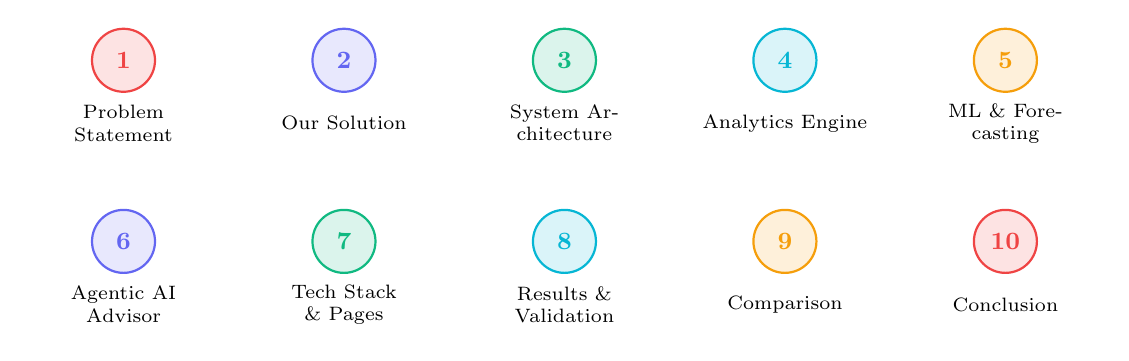
\begin{tikzpicture}
  \foreach \i/\txt/\col in {
    1/Problem Statement/ppRed,
    2/Our Solution/ppAccent,
    3/System Architecture/ppGreen,
    4/Analytics Engine/ppCyan,
    5/ML \& Forecasting/ppAmber%
  } {
    \pgfmathsetmacro{\x}{(\i-1)*2.8}
    \node[circle, draw=\col, thick, fill=\col!15, minimum size=0.8cm, font=\bfseries\small] at (\x, 0) {\textcolor{\col}{\i}};
    \node[font=\scriptsize, text width=2.2cm, align=center] at (\x, -0.8) {\txt};
  }
  \foreach \i/\txt/\col in {
    6/Agentic AI Advisor/ppAccent,
    7/Tech Stack \& Pages/ppGreen,
    8/Results \& Validation/ppCyan,
    9/Comparison/ppAmber,
    10/Conclusion/ppRed%
  } {
    \pgfmathsetmacro{\x}{(\i-6)*2.8}
    \node[circle, draw=\col, thick, fill=\col!15, minimum size=0.8cm, font=\bfseries\small] at (\x, -2.3) {\textcolor{\col}{\i}};
    \node[font=\scriptsize, text width=2.2cm, align=center] at (\x, -3.1) {\txt};
  }
\end{tikzpicture}
\end{center}
\end{frame}

% ═══════════════════ PROBLEM ═══════════════════
\begin{frame}{The Problem: Why We Built PaisaPro.ai}
\begin{columns}[T]
\column{0.52\textwidth}

\vspace{0.2cm}
\begin{center}
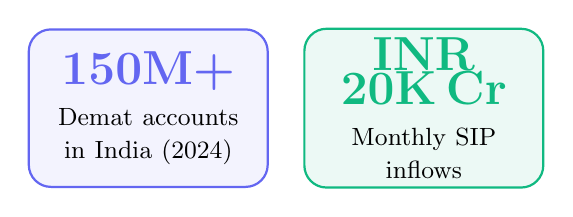
\begin{tikzpicture}
  \node[kpi=ppAccent] at (0, 0) {
    {\LARGE\bfseries\textcolor{ppAccent}{150M+}}\\[0.1cm]
    {\small Demat accounts}\\{\small in India (2024)}
  };
  \node[kpi=ppGreen] at (3.5, 0) {
    {\LARGE\bfseries\textcolor{ppGreen}{\textrm{\textbf{INR}} 20K Cr}}\\[0.1cm]
    {\small Monthly SIP}\\{\small inflows}
  };
\end{tikzpicture}
\end{center}

\vspace{0.3cm}
{\small Yet retail investors lack institutional-grade analytical tools.}

\column{0.45\textwidth}
\begin{alertblock}{Three Critical Gaps}
\begin{enumerate}
  \item \textbf{Analytics Gap}\\
  {\scriptsize ARIMA, GARCH, Fama-French require deep expertise}
  \item \textbf{AI Advisory Gap}\\
  {\scriptsize LLMs lack live data \& portfolio context}
  \item \textbf{Tool Fragmentation}\\
  {\scriptsize Screener + TradingView + Groww + ChatGPT}
\end{enumerate}
\end{alertblock}

\vspace{0.1cm}
\begin{center}
  \fcolorbox{ppRed}{ppRed!5}{\parbox{5.5cm}{\centering\small
    \textcolor{ppRed}{\textbf{No single platform unifies all of these}}
  }}
\end{center}
\end{columns}
\end{frame}

% ═══════════════════ SOLUTION ═══════════════════
\begin{frame}{Our Solution: Four Pillars}
\begin{center}
\begin{tikzpicture}
  % Pillar 1
  \node[card=ppAccent, minimum height=3.4cm] (q) at (0,0) {
    {\Large\textcolor{ppAccent}{\faChartLine}}\\[0.15cm]
    {\bfseries Quantitative\\Finance}\\[0.1cm]
    \tiny ARIMA $\cdot$ GARCH\\
    \tiny Fama-French 4-Factor\\
    \tiny Markowitz MVO\\
    \tiny Monte Carlo (1K sims)
  };
  % Pillar 2
  \node[card=ppGreen, minimum height=3.4cm] (m) at (3.8,0) {
    {\Large\textcolor{ppGreen}{\faBrain}}\\[0.15cm]
    {\bfseries Machine\\Learning}\\[0.1cm]
    \tiny Random Forest Classifier\\
    \tiny 3-Model Regression\\
    \tiny Isolation Forest\\
    \tiny K-Means Clustering
  };
  % Pillar 3
  \node[card=ppCyan, minimum height=3.4cm] (a) at (7.6,0) {
    {\Large\textcolor{ppCyan}{\faRobot}}\\[0.15cm]
    {\bfseries Agentic\\AI Advisor}\\[0.1cm]
    \tiny Llama 3.3 70B (Groq)\\
    \tiny 4 Live Tools\\
    \tiny Portfolio Context\\
    \tiny SSE Streaming
  };
  % Pillar 4
  \node[card=ppAmber, minimum height=3.4cm] (f) at (11.4,0) {
    {\Large\textcolor{ppAmber}{\faLaptopCode}}\\[0.15cm]
    {\bfseries Full-Stack\\Platform}\\[0.1cm]
    \tiny React 19 + FastAPI\\
    \tiny 18 Pages $\cdot$ 35+ APIs\\
    \tiny Dark/Light Theme\\
    \tiny Cloud Deployed
  };

  % Foundation bar
  \draw[ppAccent, ultra thick, rounded corners] (-1.3, -2.4) -- (12.7, -2.4);
  \node[font=\small\bfseries, ppPrimary] at (5.7, -2.85) {500+ NSE Stocks $\cdot$ Daily Auto-Refresh $\cdot$ Sub-100ms Cached Responses};
\end{tikzpicture}
\end{center}
\end{frame}

% ═══════════════════ ARCHITECTURE ═══════════════════
\begin{frame}{System Architecture}
\begin{center}
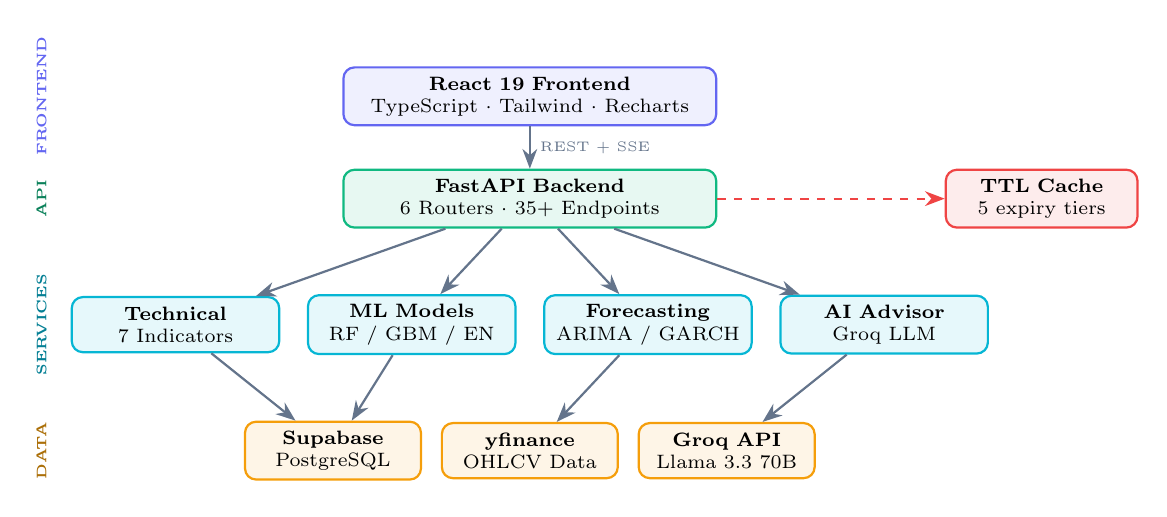
\begin{tikzpicture}[node distance=1cm]
  % Presentation layer
  \node[smallcard=ppAccent, text width=4.5cm] (fe) at (0, 3.2) {\textbf{React 19 Frontend}\\TypeScript $\cdot$ Tailwind $\cdot$ Recharts};

  % Application layer
  \node[smallcard=ppGreen, text width=4.5cm] (api) at (0, 1.9) {\textbf{FastAPI Backend}\\6 Routers $\cdot$ 35+ Endpoints};

  % Service layer
  \node[smallcard=ppCyan, text width=2.4cm] (s1) at (-4.5, 0.3) {\textbf{Technical}\\7 Indicators};
  \node[smallcard=ppCyan, text width=2.4cm] (s2) at (-1.5, 0.3) {\textbf{ML Models}\\RF / GBM / EN};
  \node[smallcard=ppCyan, text width=2.4cm] (s3) at (1.5, 0.3) {\textbf{Forecasting}\\ARIMA / GARCH};
  \node[smallcard=ppCyan, text width=2.4cm] (s4) at (4.5, 0.3) {\textbf{AI Advisor}\\Groq LLM};

  % Data layer
  \node[smallcard=ppAmber, text width=2cm] (db) at (-2.5, -1.3) {\textbf{Supabase}\\PostgreSQL};
  \node[smallcard=ppAmber, text width=2cm] (yf) at (0, -1.3) {\textbf{yfinance}\\OHLCV Data};
  \node[smallcard=ppAmber, text width=2cm] (gr) at (2.5, -1.3) {\textbf{Groq API}\\Llama 3.3 70B};

  % Cache
  \node[smallcard=ppRed, text width=2.2cm] (cache) at (6.5, 1.9) {\textbf{TTL Cache}\\5 expiry tiers};

  % Layer labels
  \node[font=\tiny\bfseries, text=ppAccent, rotate=90] at (-6.2, 3.2) {FRONTEND};
  \node[font=\tiny\bfseries, text=ppGreen!70!black, rotate=90] at (-6.2, 1.9) {API};
  \node[font=\tiny\bfseries, text=ppCyan!70!black, rotate=90] at (-6.2, 0.3) {SERVICES};
  \node[font=\tiny\bfseries, text=ppAmber!70!black, rotate=90] at (-6.2, -1.3) {DATA};

  % Arrows
  \draw[myarrow] (fe) -- node[right, font=\tiny] {REST + SSE} (api);
  \draw[myarrow] (api) -- (s1);
  \draw[myarrow] (api) -- (s2);
  \draw[myarrow] (api) -- (s3);
  \draw[myarrow] (api) -- (s4);
  \draw[myarrow] (s1) -- (db);
  \draw[myarrow] (s2) -- (db);
  \draw[myarrow] (s3) -- (yf);
  \draw[myarrow] (s4) -- (gr);
  \draw[accentarrow=ppRed, dashed] (api) -- (cache);
\end{tikzpicture}
\end{center}

\vspace{0.1cm}
\begin{center}
\footnotesize
\textbf{19 service modules} $\cdot$ Docker on HF Spaces $\cdot$ Netlify CDN $\cdot$ Supabase RLS $\cdot$ Daily cron pipeline
\end{center}
\end{frame}

% ═══════════════════ DATABASE ═══════════════════
\begin{frame}{Data Pipeline \& Database Design}
\begin{columns}[T]
\column{0.45\textwidth}
\begin{block}{Daily Refresh Pipeline}
\small
\begin{enumerate}
  \item APScheduler triggers at \textbf{6 PM IST}
  \item Clear all in-memory caches
  \item Batch-fetch OHLCV via yfinance
  \item Upsert into Supabase (500+ stocks)
  \item Compute 30+ technical indicators
  \item Refresh macro data (VIX, INR, Gold, Oil)
  \item Pre-warm analytics cache
  \item Retrain 500+ RF classifiers
\end{enumerate}
\end{block}

\column{0.52\textwidth}
\begin{block}{Database (Supabase PostgreSQL)}
\footnotesize
\renewcommand{\arraystretch}{1.2}
\begin{tabular}{@{}l l l@{}}
  \toprule
  \textbf{Table} & \textbf{PK} & \textbf{Purpose} \\
  \midrule
  stocks & symbol & Universe metadata \\
  stock\_prices & (symbol, date) & Daily OHLCV + indicators \\
  macro\_prices & (ticker, date) & VIX, INR, Gold, Oil \\
  portfolio\_holdings & id & User holdings \\
  watchlist & id & User watchlist \\
  \bottomrule
\end{tabular}
\end{block}

\vspace{0.2cm}
\begin{block}{Multi-Tier Cache (5 TTL levels)}
\footnotesize
\begin{tabular}{@{}l l@{}}
  Indices & 5 min \\
  News / Macro & 30 min \\
  Volatility / Sector & 1 hour \\
  Analytics report & 2 hours \\
  Price DataFrames / ML & 24 hours \\
\end{tabular}
\end{block}
\end{columns}
\end{frame}

% ═══════════════════ ANALYTICS ═══════════════════
\begin{frame}{Analytics Engine: 7-Indicator Composite Signals}
\begin{columns}[T]
\column{0.50\textwidth}
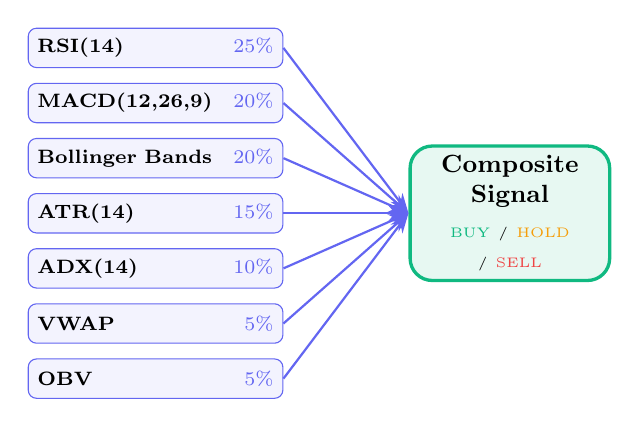
\begin{tikzpicture}
  \node[ind] (r) at (0, 4.2) {\textbf{RSI(14)} \hfill \textcolor{ppAccent}{25\%}};
  \node[ind] (m) at (0, 3.5) {\textbf{MACD(12,26,9)} \hfill \textcolor{ppAccent}{20\%}};
  \node[ind] (b) at (0, 2.8) {\textbf{Bollinger Bands} \hfill \textcolor{ppAccent}{20\%}};
  \node[ind] (a) at (0, 2.1) {\textbf{ATR(14)} \hfill \textcolor{ppAccent}{15\%}};
  \node[ind] (d) at (0, 1.4) {\textbf{ADX(14)} \hfill \textcolor{ppAccent}{10\%}};
  \node[ind] (v) at (0, 0.7) {\textbf{VWAP} \hfill \textcolor{ppAccent}{5\%}};
  \node[ind] (o) at (0, 0.0) {\textbf{OBV} \hfill \textcolor{ppAccent}{5\%}};

  \node[rectangle, rounded corners=8pt, draw=ppGreen, very thick, fill=ppGreen!10, text width=2.3cm, minimum height=1.2cm, align=center, font=\small] (sig) at (4.5, 2.1) {
    \textbf{Composite}\\
    \textbf{Signal}\\[0.05cm]
    {\tiny\textcolor{ppGreen}{BUY} / \textcolor{ppAmber}{HOLD} / \textcolor{ppRed}{SELL}}
  };

  \foreach \n in {r,m,b,a,d,v,o} {
    \draw[accentarrow] (\n.east) -- (sig.west);
  }
\end{tikzpicture}

\column{0.47\textwidth}
\begin{exampleblock}{Signal Classification}
\small
$$Score = \sum_{i=1}^{7} w_i \cdot s_i$$
\begin{itemize}
  \item $Score > +0.3$ $\rightarrow$ \textcolor{ppGreen}{\textbf{BUY}}
  \item $Score \in [-0.3, +0.3]$ $\rightarrow$ \textcolor{ppAmber}{\textbf{HOLD}}
  \item $Score < -0.3$ $\rightarrow$ \textcolor{ppRed}{\textbf{SELL}}
\end{itemize}
\end{exampleblock}

\vspace{0.15cm}
\begin{block}{Typical Distribution (Nifty 500)}
\small
\begin{tabular}{@{}lll@{}}
  \textcolor{ppGreen}{\textbf{BUY}} & 120--180 stocks & 24--36\% \\
  \textcolor{ppAmber}{\textbf{HOLD}} & 200--280 stocks & 40--56\% \\
  \textcolor{ppRed}{\textbf{SELL}} & 80--140 stocks & 16--28\% \\
\end{tabular}
\end{block}

\vspace{0.1cm}
{\scriptsize Confidence: \% of indicators agreeing (30--90\%+)}
\end{columns}
\end{frame}

% ═══════════════════ ML MODELS ═══════════════════
\begin{frame}{Machine Learning Pipeline}
\begin{columns}[T]
\column{0.48\textwidth}
\begin{block}{Random Forest Classifier}
\small
\textbf{Task:} 5-day directional prediction\\[0.1cm]
\footnotesize
\begin{tabular}{@{}ll@{}}
  Trees & 100 \\
  Training window & 252 days (1 year) \\
  Features & RSI, MACD, BB, vol ratio, etc. \\
  Accuracy & \textbf{52--58\%} (above 50\% baseline) \\
\end{tabular}
\end{block}

\vspace{0.15cm}
\begin{block}{Unsupervised Models}
\small
\textbf{K-Means} (k=4):\\
{\scriptsize Defensive $\cdot$ Value $\cdot$ Momentum $\cdot$ High-Volatility}\\[0.15cm]
\textbf{Isolation Forest:}\\
{\scriptsize Detects price spikes, volume anomalies, earnings events}
\end{block}

\column{0.48\textwidth}
\begin{block}{3-Model Regression Ensemble}
\small
\textbf{Task:} 30-day return forecasting\\[0.1cm]
\footnotesize
\begin{tabular}{@{}ll@{}}
  \textcolor{ppAccent}{\textbf{Random Forest}} & 200 trees, depth 6 \\
  \textcolor{ppGreen}{\textbf{ElasticNet}} & L1+L2, RobustScaler \\
  \textcolor{ppCyan}{\textbf{HistGBM}} & 100 est., LR 0.05 \\
\end{tabular}

\vspace{0.2cm}
\textbf{Key innovations:}
\begin{itemize}\small
  \item 32+ features (OHLC microstructure)
  \item Vol-adjusted log-return targets
  \item Walk-forward CV with embargo gap
  \item Sharpe-weighted ensemble
\end{itemize}

\vspace{0.1cm}
Directional accuracy: \textbf{55--60\%}
\end{block}
\end{columns}
\end{frame}

% ═══════════════════ FORECASTING ═══════════════════
\begin{frame}{Time-Series \& Volatility Forecasting}
\begin{columns}[T]
\column{0.48\textwidth}
\begin{block}{ARIMA Forecasting}
\small
\begin{itemize}
  \item \textbf{Stationarity:} ADF + KPSS dual tests
  \item \textbf{Grid search:} $p \in \{0..3\}$, $d \in \{0..2\}$, $q \in \{0..3\}$
  \item \textbf{Selection:} AIC minimization (48 candidates)
  \item \textbf{Output:} 30-day forecast + 95\% CI
\end{itemize}
\end{block}

\vspace{0.15cm}
\begin{block}{Holt-Winters ETS}
\small
$$\hat{y}_{t+h} = l_t + \sum_{j=1}^{h} \phi^j \cdot b_t$$
\begin{itemize}
  \item Damped additive trend
  \item Best for mean-reverting stocks
  \item Wins $\sim$30\% vs ARIMA's $\sim$60\%
\end{itemize}
\end{block}

\column{0.48\textwidth}
\begin{block}{GARCH(1,1) Volatility Model}
\small
$$\sigma_t^2 = \omega + \alpha\epsilon_{t-1}^2 + \beta\sigma_{t-1}^2$$
\begin{itemize}
  \item Captures \textbf{volatility clustering}
  \item Persistence $\alpha + \beta \approx 0.95$
  \item 30-day conditional volatility forecast
  \item MLE via \texttt{arch} library
\end{itemize}
\end{block}

\vspace{0.15cm}
\begin{exampleblock}{Volatility Regime Signals}
\footnotesize
\begin{tabular}{@{}lll@{}}
  \textcolor{ppGreen}{\textbf{LOW}} & $< 25$th pctl & $\rightarrow$ Entry signal \\
  \textcolor{ppAmber}{\textbf{NORMAL}} & 25th--75th & $\rightarrow$ Neutral \\
  \textcolor{ppRed}{\textbf{HIGH}} & 75th--95th & $\rightarrow$ Caution \\
  \textcolor{ppRed!80!black}{\textbf{EXTREME}} & $\geq 95$th & $\rightarrow$ Caution \\
\end{tabular}
\end{exampleblock}
\end{columns}
\end{frame}

% ═══════════════════ RISK & PORTFOLIO ═══════════════════
\begin{frame}{Risk Analytics \& Portfolio Optimization}
\begin{columns}[T]
\column{0.48\textwidth}
\begin{block}{Fama-French 4-Factor Model}
\small
$$R_i - R_f = \alpha + \beta_1 MKT + \beta_2 SMB + \beta_3 HML + \beta_4 MOM$$
\footnotesize
\vspace{0.1cm}
\begin{tabular}{@{}ll@{}}
  \textbf{Market} & Nifty 50 excess returns \\
  \textbf{SMB} & Small $-$ Big (size) \\
  \textbf{HML} & High $-$ Low (value) \\
  \textbf{MOM} & Winners $-$ Losers \\
\end{tabular}\\[0.15cm]
Output: $\alpha$, betas, t-stats, $R^2$
\end{block}

\vspace{0.15cm}
\begin{block}{Risk Metrics Suite}
\footnotesize
Sharpe $\cdot$ Sortino $\cdot$ Beta $\cdot$ Alpha $\cdot$ VaR(95\%) $\cdot$ Max Drawdown $\cdot$ Annualized Volatility\\[0.1cm]
Risk-free rate: \textbf{6.5\%} (10Y G-Sec yield)
\end{block}

\column{0.48\textwidth}
\begin{block}{Markowitz MVO}
\small
$$\min_{\mathbf{w}} \ \mathbf{w}^T \Sigma \mathbf{w} \quad \text{s.t.} \ \textstyle\sum w_i = 1, \ w_i \leq 0.4$$
\begin{itemize}
  \item 2,000 Monte Carlo random portfolios
  \item SLSQP constrained optimization
  \item Min-variance \& max-Sharpe identification
  \item Efficient frontier scatter visualization
\end{itemize}
\end{block}

\vspace{0.15cm}
\begin{block}{Monte Carlo Wealth Planner}
\footnotesize
\begin{itemize}
  \item 1,000 simulations per scenario
  \item SIP with annual step-up
  \item P10/P25/P50/P75/P90 bands
  \item Goal-based reverse SIP solver (binary search)
\end{itemize}
\end{block}
\end{columns}
\end{frame}

% ═══════════════════ AI ADVISOR ═══════════════════
\begin{frame}{Agentic AI Advisor --- The Key Differentiator}
\begin{center}
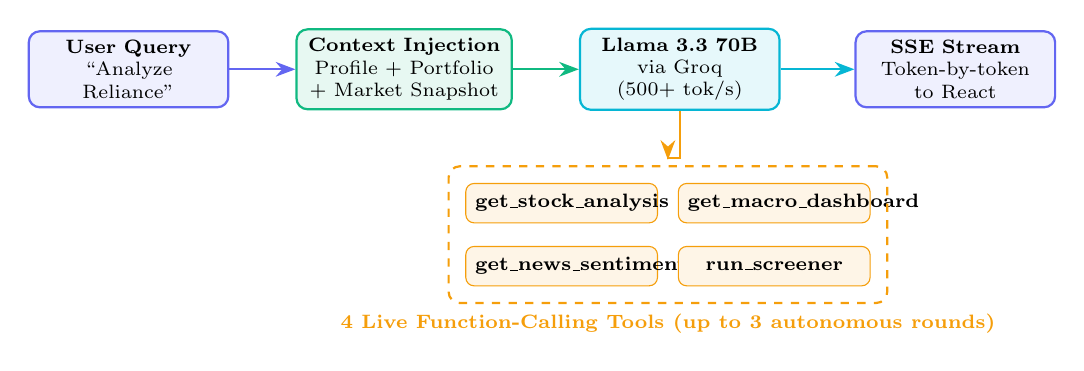
\begin{tikzpicture}
  % Flow
  \node[flowbox=ppAccent, text width=2.3cm] (user) at (0, 0) {\textbf{User Query}\\``Analyze Reliance''};
  \node[flowbox=ppGreen, text width=2.5cm] (ctx) at (3.5, 0) {\textbf{Context Injection}\\Profile + Portfolio\\+ Market Snapshot};
  \node[flowbox=ppCyan, text width=2.3cm] (llm) at (7, 0) {\textbf{Llama 3.3 70B}\\via Groq\\(500+ tok/s)};
  \node[flowbox=ppAccent, text width=2.3cm] (resp) at (10.5, 0) {\textbf{SSE Stream}\\Token-by-token\\to React};

  % Tool area
  \node[toolbox, text width=2.2cm] (t1) at (5.5, -1.7) {\textbf{get\_stock\_analysis}};
  \node[toolbox, text width=2.2cm] (t2) at (8.2, -1.7) {\textbf{get\_macro\_dashboard}};
  \node[toolbox, text width=2.2cm] (t3) at (5.5, -2.5) {\textbf{get\_news\_sentiment}};
  \node[toolbox, text width=2.2cm] (t4) at (8.2, -2.5) {\textbf{run\_screener}};

  % Arrows
  \draw[accentarrow] (user) -- (ctx);
  \draw[accentarrow=ppGreen] (ctx) -- (llm);
  \draw[accentarrow=ppCyan] (llm) -- (resp);
  \draw[accentarrow=ppAmber] (llm.south) -- ++(0,-0.6) -| (6.85,-1.15);

  % Tool boundary
  \node[draw=ppAmber, dashed, rounded corners, thick, fit=(t1)(t2)(t3)(t4), inner sep=6pt, label={[font=\scriptsize\bfseries, ppAmber]below:4 Live Function-Calling Tools (up to 3 autonomous rounds)}] {};
\end{tikzpicture}
\end{center}

\vspace{0.2cm}
\begin{columns}[T]
\column{0.48\textwidth}
\begin{block}{What Makes It ``Agentic''?}
\small
\begin{itemize}
  \item LLM \textbf{autonomously decides} when to call tools
  \item Multi-turn reasoning with tool results
  \item Portfolio-aware \textbf{personalized} advice
  \item Every recommendation backed by \textbf{live quantitative data}
\end{itemize}
\end{block}

\column{0.48\textwidth}
\begin{exampleblock}{Beyond Static RAG}
\small
\begin{itemize}
  \item Static RAG: inject data $\rightarrow$ generate
  \item \textbf{Agentic}: reason $\rightarrow$ decide tool $\rightarrow$ fetch data $\rightarrow$ synthesize $\rightarrow$ respond
  \item Inspired by Toolformer (Schick et al., 2023) and ReAct (Yao et al., 2023)
\end{itemize}
\end{exampleblock}
\end{columns}
\end{frame}

% ═══════════════════ TECH STACK ═══════════════════
\begin{frame}{Technology Stack}
\begin{columns}[T]
\column{0.30\textwidth}
\begin{block}{Backend}
\footnotesize
\renewcommand{\arraystretch}{1.15}
\begin{tabular}{@{}ll@{}}
  Python & 3.12 \\
  FastAPI & 0.111 \\
  pandas & 2.2 \\
  scikit-learn & 1.8 \\
  statsmodels & 0.14 \\
  arch & 8.0 \\
  scipy & 1.17 \\
  yfinance & 0.2 \\
  Pydantic & v2 \\
\end{tabular}
\end{block}

\column{0.30\textwidth}
\begin{block}{Frontend}
\footnotesize
\renewcommand{\arraystretch}{1.15}
\begin{tabular}{@{}ll@{}}
  React & 19 \\
  TypeScript & 5.9 \\
  Vite & 8.0 \\
  Tailwind CSS & 4 \\
  Recharts & 3.8 \\
  Zustand & 5.0 \\
  React Query & 5 \\
  React Router & 7 \\
  Axios & 1.13 \\
\end{tabular}
\end{block}

\column{0.36\textwidth}
\begin{block}{Infrastructure}
\footnotesize
\renewcommand{\arraystretch}{1.15}
\begin{tabular}{@{}ll@{}}
  Database & Supabase \\
  Backend & HF Spaces \\
  Frontend & Netlify CDN \\
  LLM & Groq Cloud \\
  Container & Docker \\
  Model & Llama 3.3 70B \\
  Scheduler & APScheduler \\
\end{tabular}
\end{block}

\vspace{0.15cm}
\begin{exampleblock}{Scale}
\footnotesize
\textbf{19} service modules\\
\textbf{6} API routers\\
\textbf{35+} endpoints\\
\textbf{18} frontend pages\\
\textbf{5-tier} TTL cache
\end{exampleblock}
\end{columns}
\end{frame}

% ═══════════════════ FRONTEND PAGES ═══════════════════
\begin{frame}{18 Interactive Pages}
\begin{columns}[T]
\column{0.30\textwidth}
{\footnotesize\textcolor{ppAccent}{\bfseries Core}}\\[0.15cm]
\small
\textcolor{ppAccent}{$\blacktriangleright$}\ Dashboard\\
\textcolor{ppAccent}{$\blacktriangleright$}\ AI Advisor Chat\\
\textcolor{ppAccent}{$\blacktriangleright$}\ Portfolio Manager\\
\textcolor{ppAccent}{$\blacktriangleright$}\ Analytics Report\\
\textcolor{ppAccent}{$\blacktriangleright$}\ Stock Screener\\
\textcolor{ppAccent}{$\blacktriangleright$}\ Portfolio Optimizer

\column{0.30\textwidth}
{\footnotesize\textcolor{ppCyan}{\bfseries Advanced Analytics}}\\[0.15cm]
\small
\textcolor{ppCyan}{$\blacktriangleright$}\ Time-Series Forecast\\
\textcolor{ppCyan}{$\blacktriangleright$}\ Volatility Forecast\\
\textcolor{ppCyan}{$\blacktriangleright$}\ Sector Rotation\\
\textcolor{ppCyan}{$\blacktriangleright$}\ Macro Dashboard\\
\textcolor{ppCyan}{$\blacktriangleright$}\ Risk Factors\\
\textcolor{ppCyan}{$\blacktriangleright$}\ ML Prediction

\column{0.30\textwidth}
{\footnotesize\textcolor{ppGreen}{\bfseries Planning \& Extras}}\\[0.15cm]
\small
\textcolor{ppGreen}{$\blacktriangleright$}\ Forward Planner\\
\textcolor{ppGreen}{$\blacktriangleright$}\ Goal Planner\\
\textcolor{ppGreen}{$\blacktriangleright$}\ Scenario Compare\\
\textcolor{ppGreen}{$\blacktriangleright$}\ News Sentiment\\
\textcolor{ppGreen}{$\blacktriangleright$}\ Model Health (MLOps)\\
\textcolor{ppGreen}{$\blacktriangleright$}\ Landing Page
\end{columns}

\vspace{0.6cm}
\begin{center}
\fcolorbox{ppGreen}{ppGreen!5}{\parbox{13cm}{\centering\small
  \cmark\ Dark/Light themes \qquad
  \cmark\ Responsive (320px -- 2560px) \qquad
  \cmark\ 7 chart types (Recharts)\\[0.1cm]
  \cmark\ SSE streaming chat \qquad
  \cmark\ Markdown rendering \qquad
  \cmark\ WCAG 2.1 AA
}}
\end{center}
\end{frame}

% ═══════════════════ RESULTS ═══════════════════
\begin{frame}{Results \& Validation}
\begin{columns}[T]
\column{0.48\textwidth}
\begin{block}{System Performance}
\footnotesize
\renewcommand{\arraystretch}{1.3}
\begin{tabular}{@{}l r@{}}
  Stocks analyzed daily & \textbf{500+} \\
  API endpoints & \textbf{35+} \\
  Frontend pages & \textbf{18} \\
  Cached response latency & \textbf{$<$ 100ms} \\
  Cold analytics build & \textbf{30--60s} \\
  LLM first token & \textbf{2--5s} \\
\end{tabular}
\end{block}

\vspace{0.1cm}
\begin{exampleblock}{Testing Results}
\footnotesize
\renewcommand{\arraystretch}{1.25}
\begin{tabular}{@{}l r@{}}
  API endpoint tests & \textbf{35/35 passed} \\
  Edge case tests & \textbf{15/15 passed} \\
  Frontend page tests & \textbf{18/18 passed} \\
  Cross-browser (6 browsers) & \textbf{All pass} \\
  Responsive breakpoints & \textbf{6/6 pass} \\
\end{tabular}
\end{exampleblock}

\column{0.48\textwidth}
\begin{block}{Model Performance}
\footnotesize
\renewcommand{\arraystretch}{1.3}
\begin{tabular}{@{}l r@{}}
  RF Classifier accuracy & \textbf{52--58\%} \\
  Regression dir.\ accuracy & \textbf{55--60\%} \\
  GARCH persistence & \textbf{$\sim$0.95} \\
  ARIMA best-model rate & \textbf{$\sim$60\%} \\
\end{tabular}
\end{block}

\vspace{0.1cm}
\begin{block}{Data Integrity}
\footnotesize
\renewcommand{\arraystretch}{1.25}
\begin{tabular}{@{}l l r@{}}
  \textbf{Metric} & \textbf{vs.} & \textbf{Dev} \\
  RSI(14) & TradingView & $<$0.5\% \\
  MACD & TradingView & $<$0.3\% \\
  BB & TradingView & $<$0.1\% \\
  Prices & Yahoo Finance & 0\% \\
\end{tabular}
\end{block}
\end{columns}
\end{frame}

% ═══════════════════ COMPARISON ═══════════════════
\begin{frame}{Comparison with Existing Platforms}
\begin{center}
\small
\renewcommand{\arraystretch}{1.15}
\begin{tabular}{@{}l c c c c c@{}}
\toprule
\textbf{Capability} & \textbf{\textcolor{ppAccent}{PaisaPro}} & \textbf{Screener.in} & \textbf{TradingView} & \textbf{Groww} & \textbf{ChatGPT} \\
\midrule
Technical Signals (7 indicators) & \cmark & \xmark & \cmark & \xmark & \xmark \\
ML Classification & \cmark & \xmark & \xmark & \xmark & \xmark \\
ML Regression Ensemble & \cmark & \xmark & \xmark & \xmark & \xmark \\
ARIMA / ETS Forecast & \cmark & \xmark & \xmark & \xmark & \xmark \\
GARCH Volatility & \cmark & \xmark & \xmark & \xmark & \xmark \\
Fama-French 4-Factor & \cmark & \xmark & \xmark & \xmark & \xmark \\
Portfolio Optimization & \cmark & \xmark & \xmark & \xmark & \xmark \\
Monte Carlo Planning & \cmark & \xmark & \xmark & \xmark & \xmark \\
AI Advisory (Live Data) & \cmark & \xmark & \xmark & \xmark & \tmark \\
Agentic Tool Use & \cmark & \xmark & \xmark & \xmark & \xmark \\
Portfolio Tracking & \cmark & \xmark & \xmark & \cmark & \xmark \\
News Sentiment & \cmark & \xmark & \xmark & \xmark & \xmark \\
\bottomrule
\end{tabular}
\end{center}

\vspace{0.3cm}
\begin{center}
  \fcolorbox{ppAccent}{ppAccent!8}{\parbox{11cm}{\centering\small
    \textcolor{ppAccent}{\textbf{PaisaPro.ai is the only platform combining all 12 capabilities in one system}}
  }}
\end{center}
\end{frame}

% ═══════════════════ LIMITATIONS ═══════════════════
\begin{frame}{Limitations \& Future Work}
\begin{columns}[T]
\column{0.48\textwidth}
\begin{alertblock}{Current Limitations}
\small
\begin{enumerate}
  \item Single-user mode (hardcoded ID)
  \item Daily OHLCV only (no intraday)
  \item Keyword-based sentiment (not FinBERT)
  \item Proxy Fama-French factors (not academic)
  \item Normal distribution in Monte Carlo
  \item LLM hallucination risk
\end{enumerate}
\end{alertblock}

\column{0.48\textwidth}
\begin{exampleblock}{Proposed Future Enhancements}
\small
\begin{enumerate}
  \item JWT multi-user authentication
  \item FinBERT transformer sentiment
  \item 5-min / 15-min intraday data
  \item Fama-French 5-factor model
  \item Options analytics (Greeks, IV)
  \item React Native mobile app
  \item Real-time WebSocket feeds
  \item Fundamental analysis (P/E, debt ratios)
  \item SEBI RIA compliance exploration
\end{enumerate}
\end{exampleblock}
\end{columns}
\end{frame}

% ═══════════════════ LESSONS LEARNED ═══════════════════
\begin{frame}{Key Lessons Learned}
\begin{columns}[T]
\column{0.48\textwidth}
\begin{block}{Engineering}
\small
\begin{itemize}
  \item \textbf{Caching is critical for UX} --- without it, 30--60s per request; with it, $<$100ms
  \item \textbf{Service-oriented modularity} --- 19 independent modules enabled rapid iteration
  \item \textbf{SSE transforms perceived performance} --- users start reading within 2s vs waiting 10--15s
\end{itemize}
\end{block}

\column{0.48\textwidth}
\begin{block}{Research}
\small
\begin{itemize}
  \item \textbf{Model simplicity wins} --- RF/GBM outperformed deep learning for daily data (250--1250 obs)
  \item \textbf{Agentic prompt engineering is iterative} --- balancing over-eager vs insufficient tool use
  \item \textbf{Financial data quality is variable} --- robust NaN handling essential for production
\end{itemize}
\end{block}
\end{columns}
\end{frame}

% ═══════════════════ CONCLUSION ═══════════════════
\begin{frame}{Conclusion}
\begin{center}
\vspace{0.2cm}
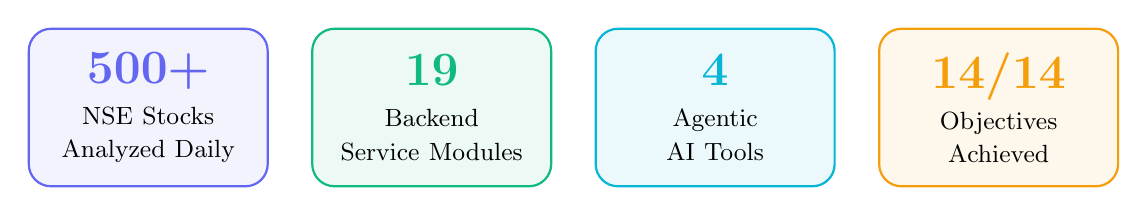
\begin{tikzpicture}
  \node[kpi=ppAccent] at (0, 0) {
    {\LARGE\bfseries\textcolor{ppAccent}{500+}}\\[0.1cm]
    {\small NSE Stocks}\\{\small Analyzed Daily}
  };
  \node[kpi=ppGreen] at (3.6, 0) {
    {\LARGE\bfseries\textcolor{ppGreen}{19}}\\[0.1cm]
    {\small Backend}\\{\small Service Modules}
  };
  \node[kpi=ppCyan] at (7.2, 0) {
    {\LARGE\bfseries\textcolor{ppCyan}{4}}\\[0.1cm]
    {\small Agentic}\\{\small AI Tools}
  };
  \node[kpi=ppAmber] at (10.8, 0) {
    {\LARGE\bfseries\textcolor{ppAmber}{14/14}}\\[0.1cm]
    {\small Objectives}\\{\small Achieved}
  };
\end{tikzpicture}
\end{center}

\vspace{0.4cm}
\begin{center}
\fcolorbox{ppAccent}{ppPrimary}{\parbox{12.5cm}{\centering
  {\large\color{white}\bfseries PaisaPro.ai demonstrates that institutional-grade}\\[0.15cm]
  {\large\color{white}\bfseries financial analytics can be democratized for}\\[0.15cm]
  {\large\color{ppCyan}\bfseries 150M+ Indian retail investors}\\[0.2cm]
  {\small\color{gray!50} through the convergence of quantitative finance, machine learning, and agentic AI}
}}
\end{center}
\end{frame}

% ═══════════════════ THANK YOU ═══════════════════
{
\setbeamertemplate{footline}{}
\setbeamercolor{background canvas}{bg=ppPrimary}
\begin{frame}[plain]
\begin{center}
\vspace{1.2cm}
{\Huge\bfseries\color{white} Thank You!}\\[0.6cm]
{\color{ppCyan}\rule{4cm}{1.5pt}}\\[0.6cm]
{\Large\color{white} Questions \& Discussion}\\[1cm]
\includegraphics[height=1.2cm]{"NMIMS logo.png"}\\[0.5cm]
{\small\color{gray!50}
  Stephen Baraik $\cdot$ Tanisha Ghosh $\cdot$ Sneha Das\\[0.2cm]
  Supervisor: Dr.\ Suresh Pathare\\[0.15cm]
  SVKM's NMIMS University $\cdot$ SOMASA $\cdot$ 2025--2026
}
\end{center}
\end{frame}
}

\end{document}
